\section{Stochastische Vorgänge: zufällige Vorgänge}
\listoftodos
\begin{bsp}
		$1$ mal würfeln. \\

		$\begin{aligned}
			 \underset{(Omega)}{\Omega} &= \text{ Menge der möglichen Ausgänge} \\
																	&= \text{ Ergebnisse } 
		\end{aligned}$
\hfill
		\begin{tikzpicture}[scale=0.7,baseline={(current bounding box.center)}]
		%	\draw[help lines] (0,0) grid (8,5);
			\draw (2,0) -- (2,5) -- (8,5) -- (8,0) -- (2,0);
			\node[rotate=0] at (3,4) {\LARGE 1};
			\node[rotate=10] at (4,3) {\LARGE 2};
			\node[rotate=-0] at (5,4) {\LARGE 3};
			\node[rotate=-0] at (6.1,2.3) {\LARGE 4};
			\node[rotate=-20] at (4.3,1.5) {\LARGE 5};
			\node[rotate=0] at (5.2,1) {\LARGE 6};
			\draw [->] (2,2.3) -- (0,2.3);
		\end{tikzpicture}

	\begin{itemize}[]
		\item% 
			\begin{flalign*}
			P(A) & = P (\text{gerade Zahlen})  \\
					 & = P(\hspace{-1.0em} \underbrace{ \set{2,4,6} }
							_{\substack{\text{Anzahl der } \\ \text{günstigen Erg.}}} \hspace{-1.0em}) 
						 = \frac{\text{Anzahl der günstigen Ergebnisse}}
							{\underbrace{\text{Anzahl der möglichen Ergebnisse}}_
							{\substack{= \text{Anzahl d. Elemente in } \Omega}}} 
						 = \frac{3}{6}\\
					 &\\
			 P (\set{1}) &= \frac{1}{6}\\ 
			\end{flalign*}	
	\end{itemize}
\todor[test]

\begin{minipage}{0.4\linewidth}
	\begin{tikzpicture}[scale=0.7]
		%\draw[help lines] (0,0) grid (8,5);
		% Box mit Omega
		\draw (2,0.5) -- (2,4.5) -- (7.5,4.5) -- (7.5,0.5) -- (2,0.5);
		\node at (1,4.5) {\Huge $\Omega$};
		% Zahlen in der Box
		\foreach \x/\y/\n/\r in {2.7/3.5/1/0,2.9/1.8/2/5,4.7/3.5/3/7,4.7/1.2/4/-5,6.7/3.5/5/0,6.9/1.5/6/0}
		\node[rotate=\r] at (\x,\y) {\LARGE \n};
		% Zahlen ausserhalb der Box
		\foreach \x/\y/\n/\r in {2.7/3.5/1/0,2.9/1.8/2/5,4.7/3.5/3/7,4.7/1.2/4/-5,6.7/3.5/5/0,6.9/1.5/6/0}
		\ifthenelse{\equal{\n}{1} \OR \equal{\n}{3} \OR \equal{\n}{5}}%
			{\node at (\x+0.4,\y+1.6) {\LARGE \n}}%
			{\node at (\x+0.1,-0.5) {\LARGE \n}};
		% Zeichnet die Pfeile
		\foreach \x/\y/\n/\r in {2.7/3.5/1/0,2.9/1.8/2/5,4.7/3.5/3/7,4.7/1.2/4/-5,6.7/3.5/5/0,6.9/1.5/6/0}
		\ifthenelse{\equal{\n}{1} \OR \equal{\n}{3} \OR \equal{\n}{5}}%
			{\draw[thick,->] (\x,\y+0.5) -- (\x+0.34,\y+1.2)}%
			{\draw[thick,->] (\x,\y-0.5) -- (\x+0.1,-0.1)};
	\end{tikzpicture}
\end{minipage}
%
\begin{minipage}{0.6\linewidth}
	ZV $X = $ Augenzahl\\
	Wahrscheinlichkeitsverteilung
	\def \var {0.10\linewidth}
	\begin{tabular}{m{0.28\linewidth}|m{\var} m{\var}m{\var}m{\var}m{\var}m{\var}}
		\centering $x_i$  & 1 & 2 & 3 & 4 & 5 & 6 \tabularnewline
		\hline
		\centering $P(X = x_i)$ & $\frac{1}{6}$ & $\frac{1}{6}$ & $\frac{1}{6}$ 
														& $\frac{1}{6}$ & $\frac{1}{6}$ & $\frac{1}{6}$ 	
	\label{Wahrscheinlichkeitsverteilung}
	\end{tabular}
\end{minipage}
~\\	
\begin{minipage}{0.45\linewidth}
	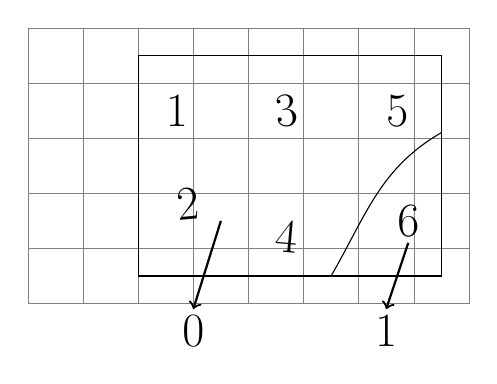
\begin{tikzpicture}[scale=0.7]
		\draw[help lines] (0,0) grid (8,5);
		% Box mit Omega
		\draw (2,0.5) -- (2,4.5) -- (7.5,4.5) -- (7.5,0.5) -- (2,0.5);
		% Zahlen in der Box
		\foreach \x/\y/\n/\r in {2.7/3.5/1/0,2.9/1.8/2/5,4.7/3.5/3/7,4.7/1.2/4/-5,6.7/3.5/5/0,6.9/1.5/6/0}
		\node[rotate=\r] at (\x,\y) {\LARGE \n};
		% Schrägstrich in der Box 
		\draw (5.5,0.5) to [out=60,in=-150] (7.5,3.1);
		% Pfeile an den Unterteilung : 0
			%definiere (lokale Variabeln)
			\def \x {3} 
			\def \y {-0.1}
		\draw[thick,->] (\x+0.5,1.5) -- (\x,\y);
		\node at (\x,\y-0.4) {\LARGE 0};
		% Pfeile an den Unterteilung : 1
			%definiere (lokale Variabeln)
			\def \x {6.5} 
			\def \y {-0.1}
		\draw[thick,->] (\x+0.4,1.1) -- (\x,\y);
		\node at (\x,\y-0.4) {\LARGE 1};
	\end{tikzpicture}
\end{minipage}
%
\begin{minipage}{0.55\linewidth}
	ZV $Y$ gibt an, ob eine $6$ gewürfelt wurde:
		\begin{itemize}[]
			\item $y_1 = 0 :$ keine $6$ wurde gewürfelt
			\item $y_2 = 1 :$ eine 6 wurde gewürfelt
		\end{itemize}
	Wahrscheinlichkeitsverteilung\\
	\begin{tabular}{c | c c}
		$y_i$ & 0 & 1\\
		\hline
		\vspace{1em} $ P( y = y_1)$ & $\frac{5}{6}$ & $\frac{1}{6}$
	\end{tabular}
\end{minipage}

\begin{minipage}{0.45\linewidth}
	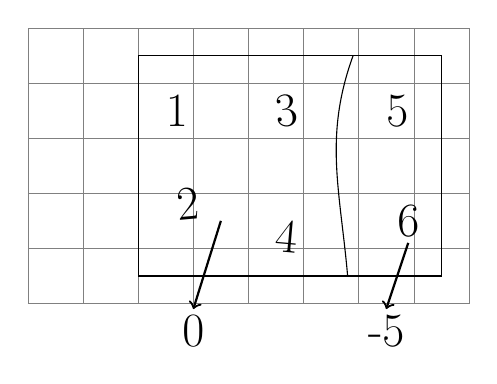
\begin{tikzpicture}[scale=0.7]
		\draw[help lines] (0,0) grid (8,5);
		% Box mit Omega
		\draw (2,0.5) -- (2,4.5) -- (7.5,4.5) -- (7.5,0.5) -- (2,0.5);
		% Zahlen in der Box
		\foreach \x/\y/\n/\r in {2.7/3.5/1/0,2.9/1.8/2/5,4.7/3.5/3/7,4.7/1.2/4/-5,6.7/3.5/5/0,6.9/1.5/6/0}
		\node[rotate=\r] at (\x,\y) {\LARGE \n};
		% Schrägstrich in der Box 
		\draw (5.8,0.5) to [out=95,in=250] (5.9,4.5);
		% Pfeile an den Unterteilung : 0
			%definiere (lokale Variabeln)
			\def \x {3} 
			\def \y {-0.1}
		\draw[thick,->] (\x+0.5,1.5) -- (\x,\y);
		\node at (\x,\y-0.4) {\LARGE 0};
		% Pfeile an den Unterteilung : 1
			%definiere (lokale Variabeln)
			\def \x {6.5} 
			\def \y {-0.1}
		\draw[thick,->] (\x+0.4,1.1) -- (\x,\y);
		\node at (\x,\y-0.4) {\LARGE -5};
	\end{tikzpicture}
\end{minipage}
%
\begin{minipage}{0.55\linewidth}
	\underline{Gewinnspiel:}
		\begin{itemize}
			\item bei $5,6 \to$ Verlust von $5EURO$
			\item bei $1,2,3$ oder $4$ Gewinn in Höhe der doppelten Augenzahl 
		\end{itemize}
	ZV $Z =$ Gewinn / Verlust in EURO\\
	Realisationsmöglichkeiten: $-5,2,4,6,8$\\
	\begin{tabular}{c | c c}
		$y_i$ & 0 & 1\\
		\hline
		\vspace{1em} $ P( y = y_1)$ & $\frac{5}{6}$ & $\frac{1}{6}$
	\end{tabular}
\end{minipage}
\end{bsp}
